%!TEX root = ../thesis.tex
%*******************************************************************************
%****************************** Third Chapter **********************************
%*******************************************************************************
\chapter{PENGUJIAN DAN ANALISA SISTEM}

% **************************** Define Graphics Path **************************
\ifpdf
    \graphicspath{{Chapter4/Figs/tinggi/}{Chapter4/Figs/idv/}{Chapter4/Figs/}}
\else
    \graphicspath{{Chapter4/Figs/Vector/}{Chapter4/Figs/}}
\fi
Pada BAB ini akan dijelaskan mengenai proses pengujian dan hasil yang didapat dari pengujian sistem tersebut.~Pengujian sistem yang dilakukan meliputi: 
\begin{itemize}
	\item Pengujian pemilihan fokus daerah kerja atau \textit{Region of Interest} (ROI).
	\item Pengujian penguatan \textit{magnification} video dengan teknik EVM \textit{(Eulerian Video Magnification)}.
	\item Pengujian ekstraksi sinyal video dengan menggunakan nilai piksel rata-rata.
	\item Pengujian nilai detak jantung dari hasil ekstraksi sinyal.
\end{itemize}

%pengambilan video, proses pengolahan data serta kumpulan data hasil uji coba.

%\section{Pengambilan video pada bagian tubuh yang dapat menunjukkan aktifitas aliran darah dan pernapasan}
%Pada proses pengujian ini dilakukan pengambilan video pada bagian tubuh tertentu, seperti pada wajah, pergelangan tangan, dan pada daerah leher menggunakan kamera DSLR (\textit{Digital Single-Lens Reflex}).
%\subsection{Tujuan}
%Pengujian pengambilan video bertujuan untuk mengumpulkan data yang berkaitan dengan perubahan karakteristik pada bagian tubuh tertentu yang menunjukkan adanya aktifitas aliran darah ataupun pernapasan, seperti pada wajah, pergelangan tangan, dan pada daerah leher.
%
%\subsection{Peralatan}
%Peralatan yang digunakan dalam proses pengujian ini adalah kamera sebagai sensor citra utama yang digunakan untuk pengambilan data berupa video, serta tripod atau penyangga kamera untuk menjaga posisi kamera agar tetap stabil saat proses pengambilan data berlangsung.
%
%%\begin{itemize}
%%	\item Kamera sebagai sensor citra utama untuk merekam video. Pada pengujian ini digunakan kamera DSLR.
%%	\item Tripod atau penyangga kamera untuk menajaga posisi kamera agar tetap stabil.
%%\end{itemize}
%
%\subsection{Prosedur}
%Prosedur yang harus dilakukan adalah sebagai berikut:
%\begin{itemize}
%	\item Pastikan tingkat pencahayaan yang ada cukup, sehingga saat melakukan proses perekaman detil-detil gambar yang dihasilkan tetap terlihat.
%	\item Tentukan bagian tubuh yang akan direkam dan pastikan terdapat aktifitas aliran darah ataupun pernapasan pada daerah tersebut. 
%	\item Atur posisi kamera dengan bagian tubuh tersebut sedemikian hingga posisinya sejajar dengan letak kamera.
%	\item Pastikan posisi kamera tetap dan stabil sehingga tidak terjadi gangguan berupa perubahan posisi kamera.
%	\item Lakukan proses pengambilan video dengan waktu yang cukup ---lebih dari 10 detik---.  
%\end{itemize}


\section{Pengujian Pemilihan ROI}
Pada proses pengujian ini terlebih dahulu dilakukan pengambilan data berupa video pada bagian tubuh tertentu, seperti pada wajah, pergelangan tangan, dan pada daerah leher menggunakan kamera DSLR (\textit{Digital Single-Lens Reflex}).~Hasil pengambilan data tersebut kemudian akan digunakan sebagai masukan \textit{input} untuk pemilihan daerah kerja atau ROI.
\subsection{Tujuan}
Pengujian pemilihan ROI bertujuan untuk menentukan fokus daerah kerja yang akan digunakan untuk menjalankan proses-proses berikutnya.~Daerah kerja yang dimaksud adalah bagian dari tubuh yang menunjukkan adanya aktifitas aliran darah ataupun pernapasan.~Pemilihan ROI dapat mempengaruhi kualitas dan tingkat keakuratan data yang dihasilkan.

%Pengujian pengambilan video bertujuan untuk mengumpulkan data yang berkaitan dengan perubahan karakteristik pada bagian tubuh tertentu yang menunjukkan adanya aktifitas aliran darah ataupun pernapasan, seperti pada wajah, pergelangan tangan, dan pada daerah leher.

\subsection{Peralatan}
Peralatan yang digunakan dalam proses pengujian ini adalah kamera sebagai sensor citra utama yang digunakan untuk pengambilan data berupa video, serta tripod atau penyangga kamera untuk menjaga posisi kamera agar tetap stabil saat proses pengambilan data berlangsung. \textit{Software} MATLAB digunakan sebagai alat bantu pemrosesan citra digital untuk menentukan daerah ROI pada data video.

%\begin{itemize}
%	\item Kamera sebagai sensor citra utama untuk merekam video.~Pada pengujian ini digunakan kamera DSLR.
%	\item Tripod atau penyangga kamera untuk menajaga posisi kamera agar tetap stabil.
%\end{itemize}

\subsection{Prosedur}
Prosedur yang harus dilakukan adalah sebagai berikut:
\begin{itemize}
	\item Pastikan tingkat pencahayaan yang ada cukup, sehingga saat melakukan proses perekaman detil-detil gambar yang dihasilkan tetap terlihat.
	\item Tentukan bagian tubuh yang akan direkam dan pastikan terdapat aktifitas aliran darah ataupun pernapasan pada daerah tersebut.~
	\item Atur posisi kamera dengan bagian tubuh tersebut sedemikian hingga posisinya sejajar dengan letak kamera.
	\item Pastikan posisi kamera tetap dan stabil sehingga tidak terjadi gangguan berupa perubahan posisi kamera.
	\item Atur kamera untuk merekam dengan nilai \textit{frame rate} lebih dari 20 \textit{frame} tiap detiknya.
	\item Lakukan proses pengambilan video dengan waktu yang cukup ---lebih dari 8 detik---.
\end{itemize}

\subsection{Hasil dan Analisa}
Pada pengujian kali ini pemilihan ROI dilakukan secara manual, yaitu dengan cara mendefinisikan terlebih dahulu bagian-bagian tubuh yang dapat menunjukkan aktifitas aliran darah ataupun pernapasan.~Berikut adalah hasil dari proses pengujian yang didapat.

\begin{figure}[ht]
	\vspace{0.5em}
	\centering
	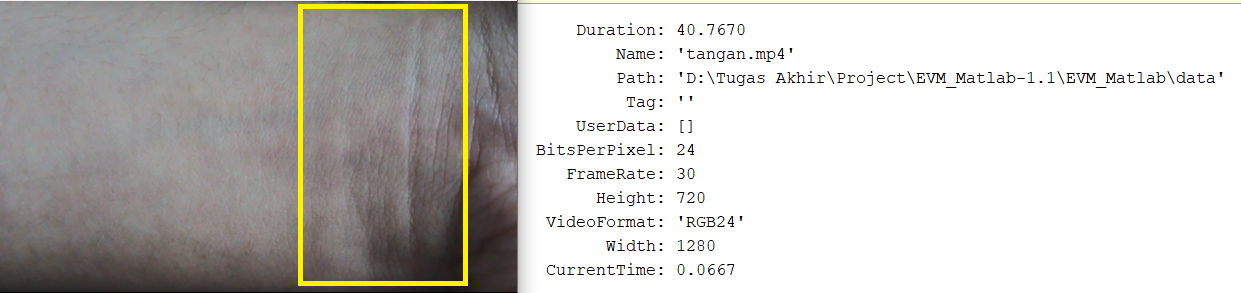
\includegraphics[width=\textwidth]{tangan1_roi}
	\caption{Data cuplikan video tangan kiri dengan ROI.}
	\label{fig:tangan1}   
\end{figure}
Pada Gambar~\ref{fig:tangan1} merupakan cuplikan gambar dari data rekaman sampel tangan kiri yang selanjutnya akan disebut dengan data "Tangan1".~Sebelum melakukan pengambilan data, telah dilakukan pengecekan terlebih dahulu pada daerah pergelangan tangan untuk memastikan adanya area yang menunjukkan aktifitas aliran darah.~Pada area yang dibatasi dengan kotak berwarna kuning, terdapat urat nadi yang dapat merepresentasikan aktifitas aliran darah pada tubuh, khususnya pergelangan tangan.~Akan tetapi, saat diamati dengan pengelihatan biasa ataupun dalam proses pengambilan data video "Tangan1" pergerakan nadi yang terjadi tidak terlihat dengan jelas.

\begin{figure}[ht]
	\vspace{0.5em}
	\centering
	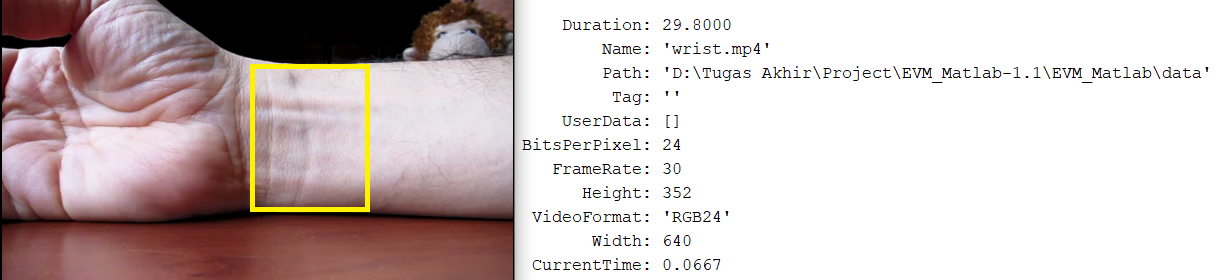
\includegraphics[width=\textwidth]{tangan2_roi}
	\caption{Data cuplikan video tangan kanan dengan ROI.}
	\captionsetup{font={footnotesize}}  
	\caption*{sumber: people.csail.mit.edu/mrub/vidmag/}
	\label{fig:tangan2}   
\end{figure}
 Gambar~\ref{fig:tangan2} merupakan cuplikan gambar dari data rekaman sampel tangan kanan yang didapatkan dari dataset penelitian \citet{Wu2012} dan \citet{RubinsteinPhDThesis2014} yang selanjutnya akan disebut dengan data "Tangan2".~Berdasarkan penjelasan yang didapatkan dari penelitian tersebut, daerah fokus kerja yang menunjukkan aktifitas pergerakan nadi ditandai dengan kotak berwarna kuning.~Seperti halnya pada data "Tangan1", data "Tangan2" tidak terlihat dengan kasat mata pergerakan nadi yang terjadi.

\begin{figure}[ht]
	\vspace{0.5em}
	\centering
	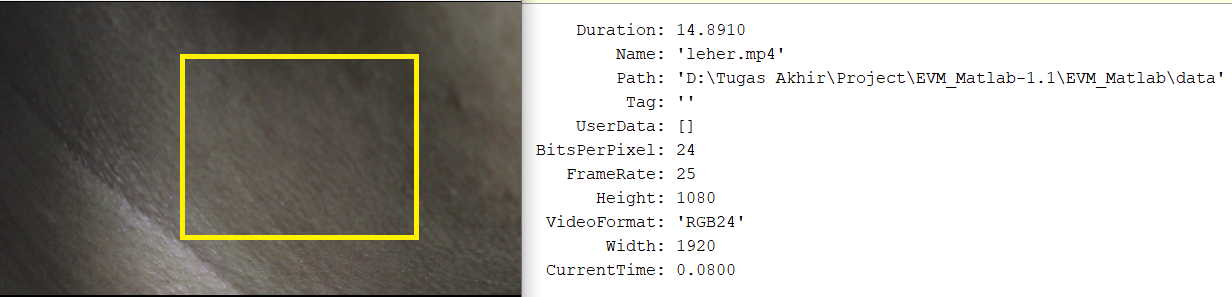
\includegraphics[width=\textwidth]{leher1_roi}
	\caption{Data cuplikan video leher kiri dengan ROI.}
	\label{fig:leher1}   
\end{figure}
 Terlihat pada Gambar~\ref{fig:leher1} data dari rekaman sampel yang diambil pada bagian leher sebelah kiri yang selanjutnya akan disebut dengan data "Leher1".~Pada area fokus kerja yang ditandai dengan kotak berwarna kuning, terdapat pergerakan nadi yang terjadi dan dapat telihat ketika diamati dengan pengelihatan biasa meskipun perubahannya tidak terlalu signifikan namun tampak jika dibandingkan dengan pergerakan nadi di daerah pergelangan tangan.
\newpage
\begin{figure}[ht]
	\vspace{0.5em}
	\centering
	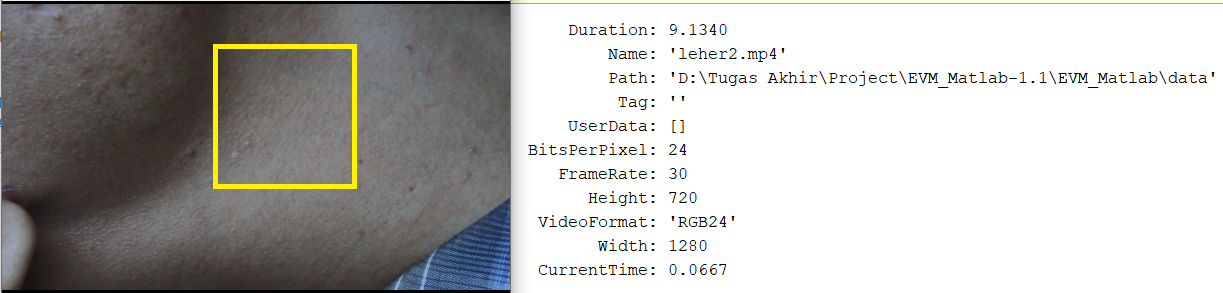
\includegraphics[width=\textwidth]{leher2_roi}
	\caption{Data cuplikan video leher kanan dengan ROI.}
	\label{fig:leher2}   
\end{figure}
Gambar~\ref{fig:leher2} merupakan data rekaman sampel yang diambil dari bagian leher sebelah kanan yang selanjutnya akan disebut sebagai data "Leher2".~Data "Leher2" ini memiliki karakteristik yang identik dengan data "Leher1" di mana terlihat aktifitas nadi yang ditandai dengan kotak berwarna kuning.~Akan tetapi, pergerakan nadi yang terjadi pada data "Leher1" lebih terlihat dan cakupan areanya lebih luas jika dibandingkan dengan data "Leher2".~Hal tersebut dapat dipengaruhi oleh beberapa faktor seperti jarak pengambilan data, tingkat pencahayaan, maupun perbedaan karakteristik dari masing-masing individu.

\begin{figure}[ht]
	\vspace{0.5em}
	\centering
	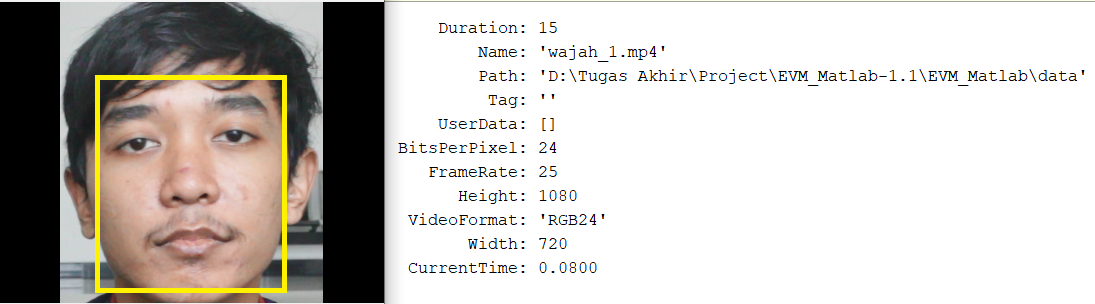
\includegraphics[width=\textwidth]{wajah1_roi}
	\caption{Data cuplikan video wajah subyek1 dengan ROI.}
	\label{fig:wajah1}   
\end{figure}
Pada Gambar~\ref{fig:wajah1} tampak cuplikan data dari sampel rekaman video yang diambil pada daerah sekitar wajah yang selanjutnya akan disebut dengan data "Wajah1".~Pengambilan data pada daerah wajah dilakukan karena karakteristik kulit pada daerah ini yang lebih reflektif terhadap cahaya.~Hal tersebut telah dijelaskan sebelumnya pada penelitian yang dilakukan oleh \citet{Poh2010,Poh2011}, serta Sun dan Thakor \citep{sun2016}.~Oleh karena itu, area fokus kerja atau ROI yang digunakan meliputi hampir keseluhuran daerah wajah.
\newpage
\begin{figure}[ht]
	\vspace{0.5em}
	\centering
	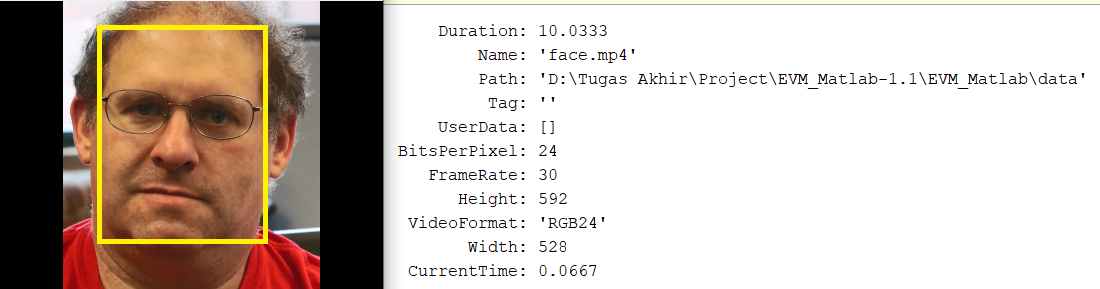
\includegraphics[width=\textwidth]{wajah2_roi}
	\caption{Data cuplikan video wajah subyek2 dengan ROI.}
	\captionsetup{font={footnotesize}}  
	\caption*{sumber: people.csail.mit.edu/mrub/vidmag/}
	\label{fig:wajah2}   
\end{figure}
Gambar~\ref{fig:wajah2} merupakan cuplikan dari dataset rekaman sampel wajah yang digunakan dalam penelitian \citet{Wu2012} dan \citet{RubinsteinPhDThesis2014} yang selanjutnya akan disebut dengan data "Wajah2".~Seperti halnya pada data "Wajah1", kotak kuning yang menandakan daerah fokus kerja pada data "Wajah2" mencangkup hampir seluruh bagian wajah.

\begin{figure}[ht]
	\vspace{0.5em}
	\centering
	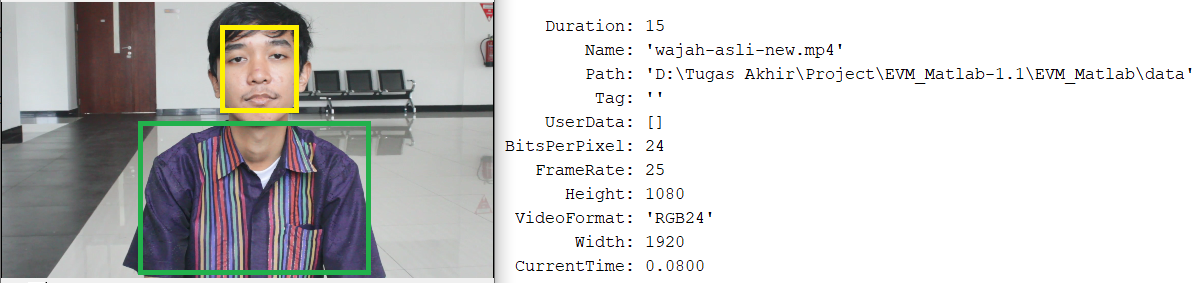
\includegraphics[width=\textwidth]{badan_roi}
	\caption{Data cuplikan video bagian tubuh atas dengan ROI.}
	\label{fig:badan}   
\end{figure}
Gambar~\ref{fig:badan} menunjukkan cuplikan sampel data dari setengah badan bagian atas yang terdiri dari bagian wajah dan badan yang selanjutnya disebut dengan data "Badan".~Pada data "Badan" terdapat dua area fokus kerja yang ditandai dengan kotak dengan warna yang berbeda.~Kotak warna kuning menandakan area fokus yang digunakan untuk menentukan nilai detak jantung seperti yang dilakukan pada data-data sebelumnya yang memiliki warna kotak yang serupa, sedangkan kotak berwarna hijau digunakan untuk menghitung tingkat pernapasan dari subyek.

\newpage
\section{Pengujian magnifikasi video dengan teknik EVM \textit{(Eulerian Video Magnification)}}
Pada pengujian ini dilakukan proses penguatan dalam artian menguatkan informasi-informasi yang terdapat pada data-data yang telah diperoleh dalam proses sebelumnya dengan menggunakan teknik EVM yang dirumuskan dalam penelitian \citet{Wu2012} dan \citet{RubinsteinPhDThesis2014}.

\subsection{Tujuan}
Pengujian ini bertujuan untuk memperjelas informasi-informasi yang terdapat pada data-data video yang telah dijelaskan sebelumnya.~Dalam pengujian ini, informasi yang akan diperjelas adalah informasi yang berkaitan tentang aktifitas dari bagian-bagian pada tubuh yang dapat menunjukkan adanya aktifitas aliran darah dan pernapasan.

\subsection{Peralatan}
Peralatan yang digunakan dalam pengujian ini adalah \textit{software} MATLAB dengan tambahan \textit{library} \textit{(Eulerian Video Magnification)}.

\subsection{Prosedur}
Prosedur pengujian magnifikasi video yang harus dilakukan adalah sebagai berikut:
\begin{itemize}
\item Buatlah direktori baru dalam folder \textit{library} EVM yang berisikan data rekaman video yang telah didapatkan pada proses sebelumnya.
\item Buka aplikasi MATLAB dan jalankan instalasi \textit{library} EVM.~
\item Setelah proses instalasi selesai, pilih data dalam \textit{folder} yang telah dibuat sebelumnya untuk diproses.
\item Atur parameter-parameter yang ada yaitu nilai alpha, level, frekuensi bawah, frekuensi atas, sampling rate, dan chromAttenuation sesuai penjelasan yang terdapat pada sub-BAB \ref{ssec:EMM}.~
\item Jalankan program dan amati perubahan yang terjadi.~Atur nilai dari parameter di atas untuk melihat respon yang didapatkan.
\end{itemize}

\subsection{Hasil dan Analisa}
Pengujian ini dilakukan menggunakan beberapa jenis filter yang berbeda pada proses magnifikasi video dengan teknik EVM untuk melihat respon serta karakteristik dari masing-masing filter yang digunakan.
\newpage
\begin{figure}[ht]
	\vspace{0.5em}
	\centering
	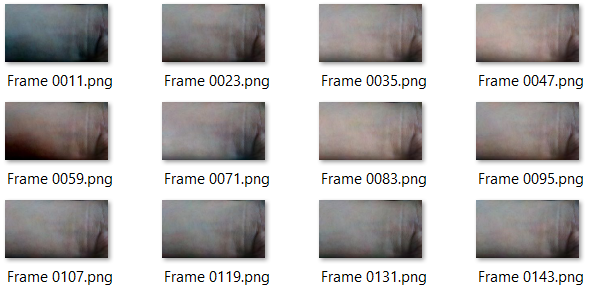
\includegraphics[width=\textwidth,height=0.4\linewidth]{data-tangan1-ideal}
	\caption{Sekuen gambar data Tangan1 dengan filter \textit{spatial-laplacian pyramid-temporal-ideal}.}
	\label{fig:sekuen-tangan1}   
\end{figure}
Gambar~\ref{fig:sekuen-tangan1} merupakan hasil dari proses amplifikasi menggunakan filter \textit{laplacian pyramid} pada domain \textit{spatial} ditambah dengan filter \textit{Ideal bandpass} dalam domain \textit{temporal}.~Hasil dari gabungan kedua filter ini memiliki karakteristik penguatan warna dan gerak.~Penguatan warna yang dihasilkan dengan filter ini lebih dominan dibandingkan penguatan gerak yang dihasilkan.~Hal tersebut terlihat pada sekuen gambar pada Gambar~\ref{fig:sekuen-tangan1}.~Hasil dari aplikasi filter ini pada data Tangan1 hanya berhasil menguatkan informasi warna namun belum berhasil untuk menguatkan informasi aktifitas nadi yang dibutuhkan untuk proses penghitungan nilai detak jantung.

\begin{figure}[ht]
	\vspace{0.5em}
	\centering
	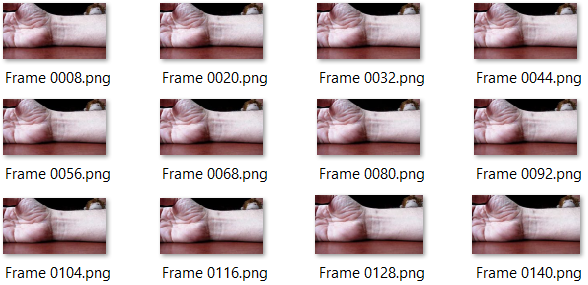
\includegraphics[width=\textwidth]{data-tangan2}
	\caption{Sekuen gambar data Tangan2 dengan filter \textit{spatial-laplacian pyramid-temporal-infinite impulse response}.}
	\label{fig:sekuen-tangan2}   
\end{figure}
Pada hasil pengujian yang ditampilkan pada Gambar~\ref{fig:sekuen-tangan2} dilakukan proses magnifikasi dengan menggunakan filter \textit{laplacian pyramid} pada domain \textit{spatial} ditambah dengan filter \textit{Second-order Infinite Impulse Response Bandpass} dalam domain \textit{temporal}.~Karakteristik dari hasil pengujian menggunakan filter tersebut pada data Tangan2 berupa penguatan gerak tanpa disertai dengan penguatan warna yang terjadi.~Hasil dari aplikasi filter ini dapat menguatkan informasi pergerakan nadi yang digunakan untuk perhitungan nilai detak jantung.~Akan tetapi, saat mengaplikasikan filter ini pada data Tangan1 hasil yang didapatkan tidak sebaik hasil pada data Tangan2.~Pada data Tangan1 informasi pergerakan urat nadi masih tidak dapat terlihat dengan jelas.

\begin{figure}[ht]
	\vspace{0.5em}
	\centering
	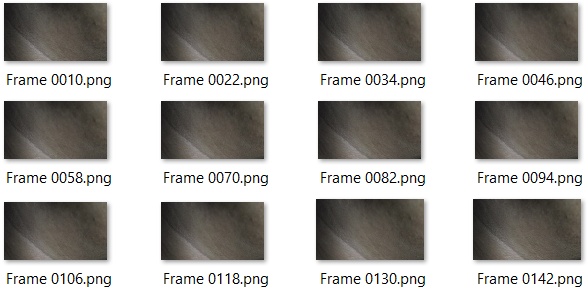
\includegraphics[width=\textwidth]{data-leher1}
	\caption{Sekuen gambar data Leher1 dengan filter \textit{spatial-laplacian pyramid-temporal-infinite impulse response}.}
	\label{fig:sekuen-leher1}   
\end{figure}
Gambar~\ref{fig:sekuen-leher1} merupakan hasil dari proses magnifikasi dari data Leher1 dengan menggunakan filter \textit{laplacian pyramid} pada domain \textit{spatial} ditambah dengan filter \textit{Second-order Infinite Impulse Response Bandpass} dalam domain \textit{temporal}.~Sama seperti pengujian sebelumnya pada data Tangan2, didapatkan karakteristik filter ini hanya menguatkan informasi gerak tanpa adanya penguatan informasi warna.~Hasil dari penggunaan filter ini dapat memperkuat informasi pergerakan nadi di daerah leher pada data Leher1 di mana sebelum proses penggunan filter aktifitas pergerakan nadi sudah terlihat meskipun tidak signifikan.
\newpage
\begin{figure}[ht]
	\vspace{0.5em}
	\centering
	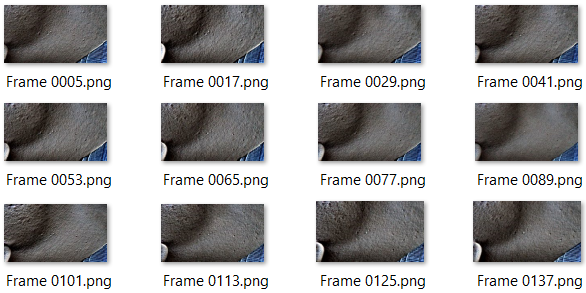
\includegraphics[width=\textwidth]{data-leher2}
	\caption{Sekuen gambar data Leher2 dengan filter \textit{spatial-laplacian pyramid-temporal-infinite impulse response}.}
	\label{fig:sekuen-leher2}   
\end{figure}

Pada Gambar~\ref{fig:sekuen-leher2} merupakan hasil dari proses magnifikasi pada data Leher2 dengan menggunakan filter yang sama seperti pada Gambar~\ref{fig:sekuen-leher1} yaitu filter \textit{laplacian pyramid} pada domain \textit{spatial} ditambah dengan filter \textit{Second-order Infinite Impulse Response Bandpass} dalam domain \textit{temporal}.~Perbedaan dari pengujian data Leher1 dan Leher2 ini adalah nilai dari parameter-parameter yang digunakan, di mana nilai parameter dari data Leher2 diatur dengan nilai yang lebih tinggi dibandingkan dengan nilai dari parameter data Leher1.~Berdasarkan hasil yang didapatkan dari pengujian ini diketahui bahwa penguatan yang terjadi pada data Leher2 lebih besar dibandingkan pada data Leher1 sehingga aktifitas nadi yang tampak pada data Leher2 dalam Gambar~\ref{fig:sekuen-leher2} lebih terlihat jelas dibandingkan data Leher1 pada Gambar~\ref{fig:sekuen-leher1}.~Namun, dengan menaikkan nilai parameter magnifikasi, artefak gerak yang ditemukan menjadi semakin banyak.
\newpage
\begin{figure}[ht]
	\vspace{0.5em}
	\centering
	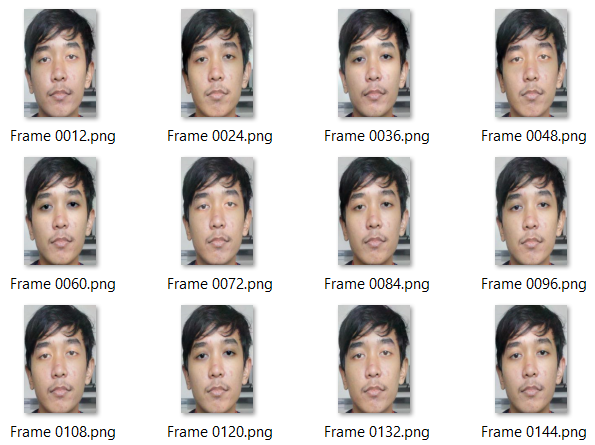
\includegraphics[width=\textwidth,height=0.5\linewidth]{data-wajah1}
	\caption{Sekuen gambar data Wajah1 dengan filter \textit{spatial-gaussian pyramid-temporal-ideal}.}
	\label{fig:sekuen-wajah1}   
\end{figure}
Gambar~\ref{fig:sekuen-wajah1} merupakan hasil dari proses magnifikasi data Wajah1 dengan menggunakan filter \textit{Gaussian pyramid} pada domain \textit{spatial} ditambah dengan filter \textit{Ideal Bandpass} dalam domain \textit{temporal}.~Hasil dari kombinasi kedua filter ini memiliki karakteristik penguatan gerak serta penguatan pada informasi warna gambar yang cukup signifikan. Berdasarkan hasil pengujian pada data Wajah1 yang terlihat pada Gambar~\ref{fig:sekuen-wajah1} perbedaan terutama pada informasi warna yang paling tampak secara visual terlihat berada pada daerah sekitar mata.

\begin{figure}[ht]
	\vspace{0.5em}
	\centering
	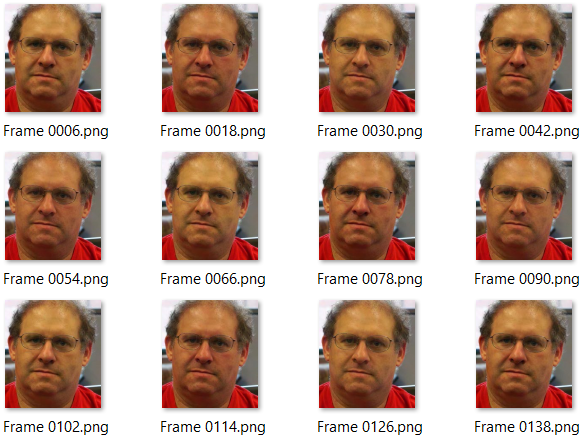
\includegraphics[width=\textwidth,height=0.4\linewidth]{data-wajah2}
	\caption{Sekuen gambar data Wajah1 dengan filter \textit{spatial-gaussian pyramid-temporal-ideal}.}
	\label{fig:sekuen-wajah2}   
\end{figure}
Hasil pengujian proses magnifikasi data Wajah2 pada Gambar~\ref{fig:sekuen-wajah2} dengan menggunakan filter yang sama dengan pengujian sebelumnya pada Gambar~\ref{fig:sekuen-wajah1} yaitu dengan filter \textit{Gaussian pyramid} pada domain \textit{spatial} ditambah dengan filter \textit{Ideal Bandpass} dalam domain \textit{temporal}.~Dari hasil pengujian, didapatkan sedikit perbedaan karakteristik yang ditemukan pada Gambar~\ref{fig:sekuen-wajah1} dan Gambar~\ref{fig:sekuen-wajah2} di mana pada data Wajah2 perubahan warna yang signifikan ditunjukkan pada daerah kulit, sedangkan pada data Wajah1 perubahan warna yang signifikan terlihat pada area mata.~Hal tersebut dapat terjadi akibat pengaruh dari beberapa faktor seperti jarak pengambilan data, tingkat pencahayaan, atau perbedaan karakteristik dari masing-masing individu.


\begin{figure}[ht]
	\vspace{0.5em}
	\centering
	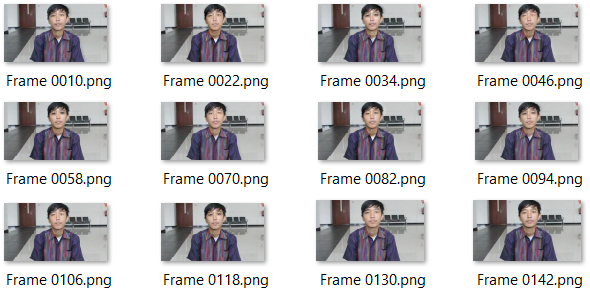
\includegraphics[width=\textwidth]{data-badan}
	\caption{Sekuen gambar data Badan dengan filter \textit{spatial-gaussian pyramid-temporal-ideal}.}
	\label{fig:sekuen-badan}   
\end{figure}
Gambar~\ref{fig:sekuen-badan} merupakan hasil dari proses magnifikasi dengan menggunakan filter yang sama dengan filter yang digunakan pada Gambar~\ref{fig:sekuen-wajah1} dan Gambar~\ref{fig:sekuen-wajah2}.~Perbedaan dari pengujian ini dengan pengujian sebelumnya terletak pada area fokus kerja yang digunakan, di mana pada pengujian ini area fokus yang digunakan lebih kecil dibandingkan pada pengujian sebelumnya.~Hasil yang didapatkan dari pengujian ini identik dengan hasil yang didapatkan pada Gambar~\ref{fig:sekuen-wajah1} di mana perubahan warna yang signifikan terjadi pada daerah sekitar mata.~Hal ini dikarenakan oleh subyek pengambilan data merupakan orang yang sama dan tempat serta kondisi pengambilan data yang identik.

\newpage
\section{Pengujian ekstraksi sinyal video dengan menggunakan nilai piksel rata-rata}
Pada pengujian ini dilakukan proses ekstraksi sinyal yang didapatkan dari data-data yang telah diolah sebelumnya dengan menggunakan proses magnifikasi dengan teknik EVM, khususnya pada data yang mengalami penguatan warna yaitu data Wajah1, Wajah2 dan Badan.~Ekstraksi sinyal dengan menggunakan nilai rata-rata piksel (\textit{pixel-mean-levels}) dapat dilakukan karena perubahan informasi warna yang didapatkan berpengaruh terhadap nilai rata-rata piksel dari setiap kanal RGB (\textit{Red-Green-Blue}) yang digunakan.
\subsection{Tujuan}
Pengujian ekstraksi sinyal video bertujuan untuk memperoleh karakteristik sinyal dari rata-rata nilai piksel yang dihasilkan dari masing-masing kanal warna RGB.~Sinyal tersebut kemudian akan dianalisa apakah dapat digunakan untuk merepresentasikan sinyal detak jantung.

\subsection{Peralatan}
Peralatan yang digunakan dalam pengujian ini adalah \textit{software} MATLAB dengan tambahan \textit{library} \textit{(Image Acquisition Toolbox)}.
\subsection{Prosedur}
Prosedur pengujian ekstraksi sinyal yang harus dilakukan adalah sebagai berikut:
\begin{itemize}
	\item Buka aplikasi MATLAB dan tentukan direktori data yang akan diekstrak sinyalnya.
	\item Pilih data yang akan diekstrak sinyalnya, kemudian ekstrak data setiap frame dan simpan dalam \textit{folder} tersendiri.
	\item Setelah proses ekstraksi data setiap frame selesai, pisahkan setiap kanal warna RGB dan hitung rata-rata piksel dari masing-masing kanal warna pada setiap frame.
	\item Buatlah grafik pada MATLAB yang menunjukkan urutan hasil ekstraksi rata-rata piksel dengan waktu.
\end{itemize}
\newpage
\subsection{Hasil dan Analisa}

\begin{figure}[ht]
	\vspace{0.5em}
	\centering
	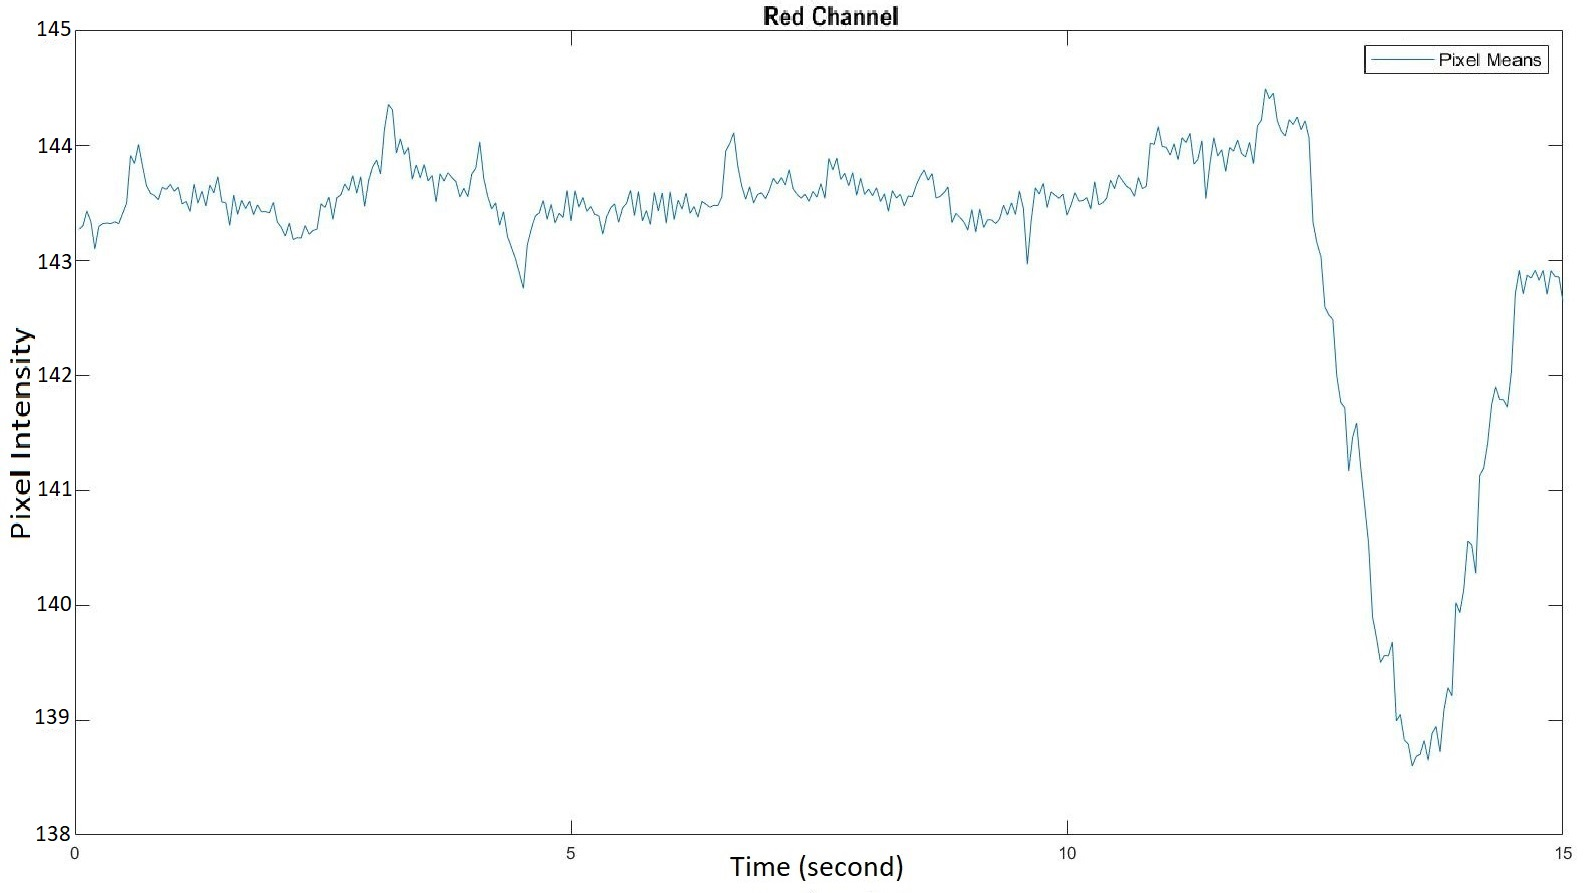
\includegraphics[width=\textwidth,height=0.25\textheight]{Red_channel_wajah1-ori}
	\caption{Grafik kanal warna merah Wajah1 sebelum proses magnifikasi.}
	\label{fig:grafik-red-wajah1}   
\end{figure}
Pada Gambar~\ref{fig:grafik-red-wajah1} terlihat bahwa hasil ekstraksi sinyal pada kanal warna merah sebelum dilakukan proses magnifikasi belum dapat merepresentasikan sinyal PPG untuk menentukan nilai rata-rata detak jantung.

\begin{figure}[ht]
	\vspace{0.5em}
	\centering
	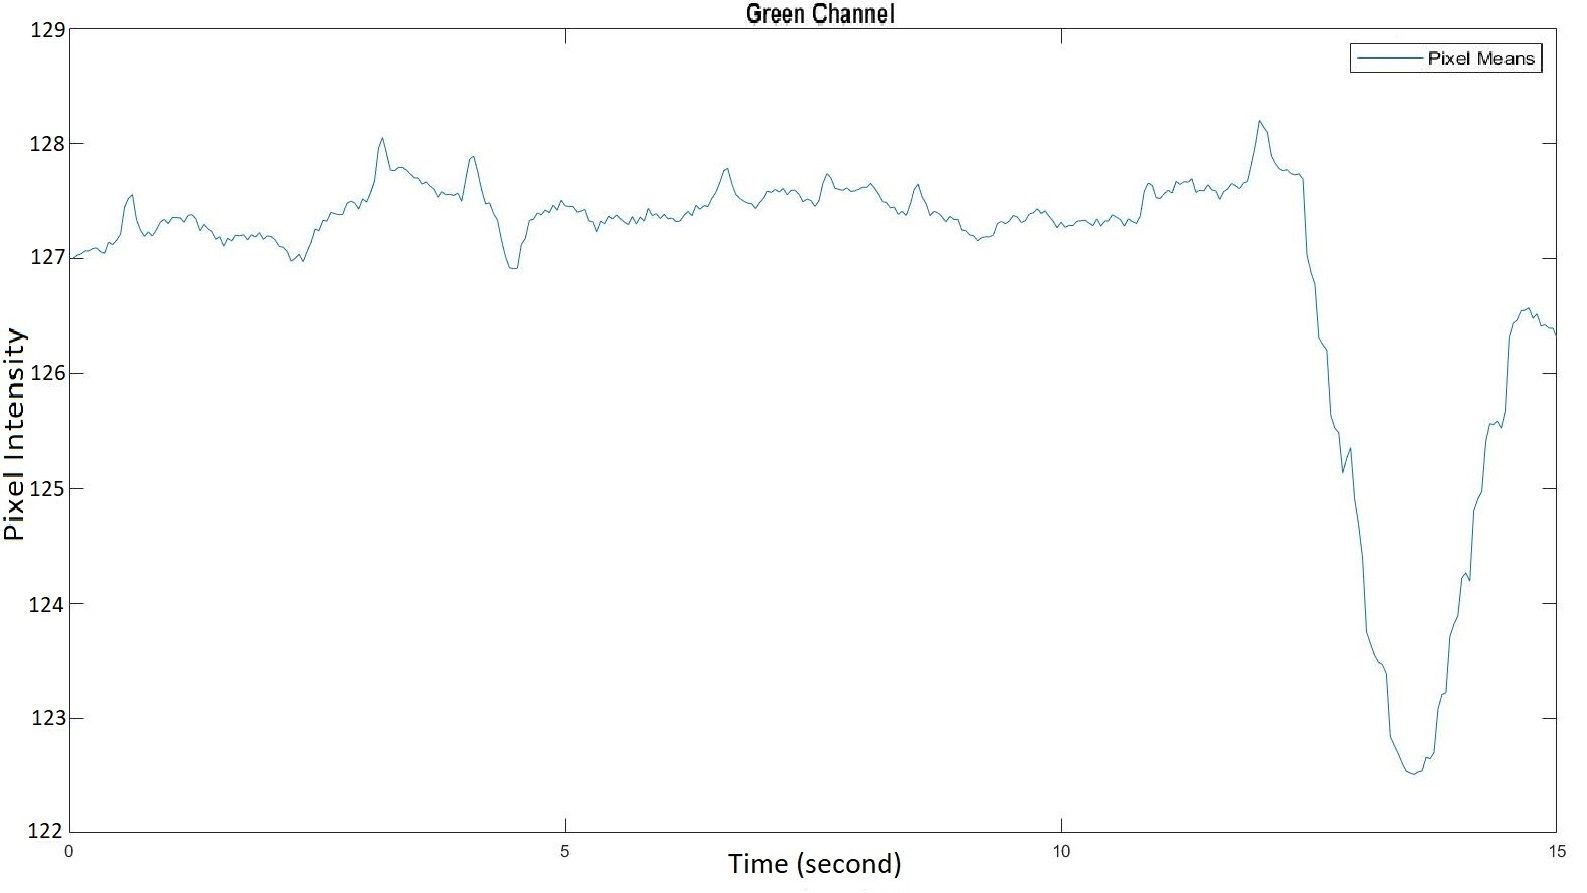
\includegraphics[width=\textwidth,height=0.25\textheight]{Green_channel_wajah1-ori}
	\caption{Grafik kanal warna hijau Wajah1 sebelum proses magnifikasi.}
	\label{fig:grafik-green-wajah1}   
\end{figure}

Pada Gambar~\ref{fig:grafik-green-wajah1} terlihat bahwa hasil ekstraksi sinyal pada kanal warna hijau sebelum dilakukan proses magnifikasi belum dapat merepresentasikan sinyal PPG untuk menentukan nilai rata-rata detak jantung.
\newpage
\begin{figure}[ht]
	\vspace{0.5em}
	\centering
	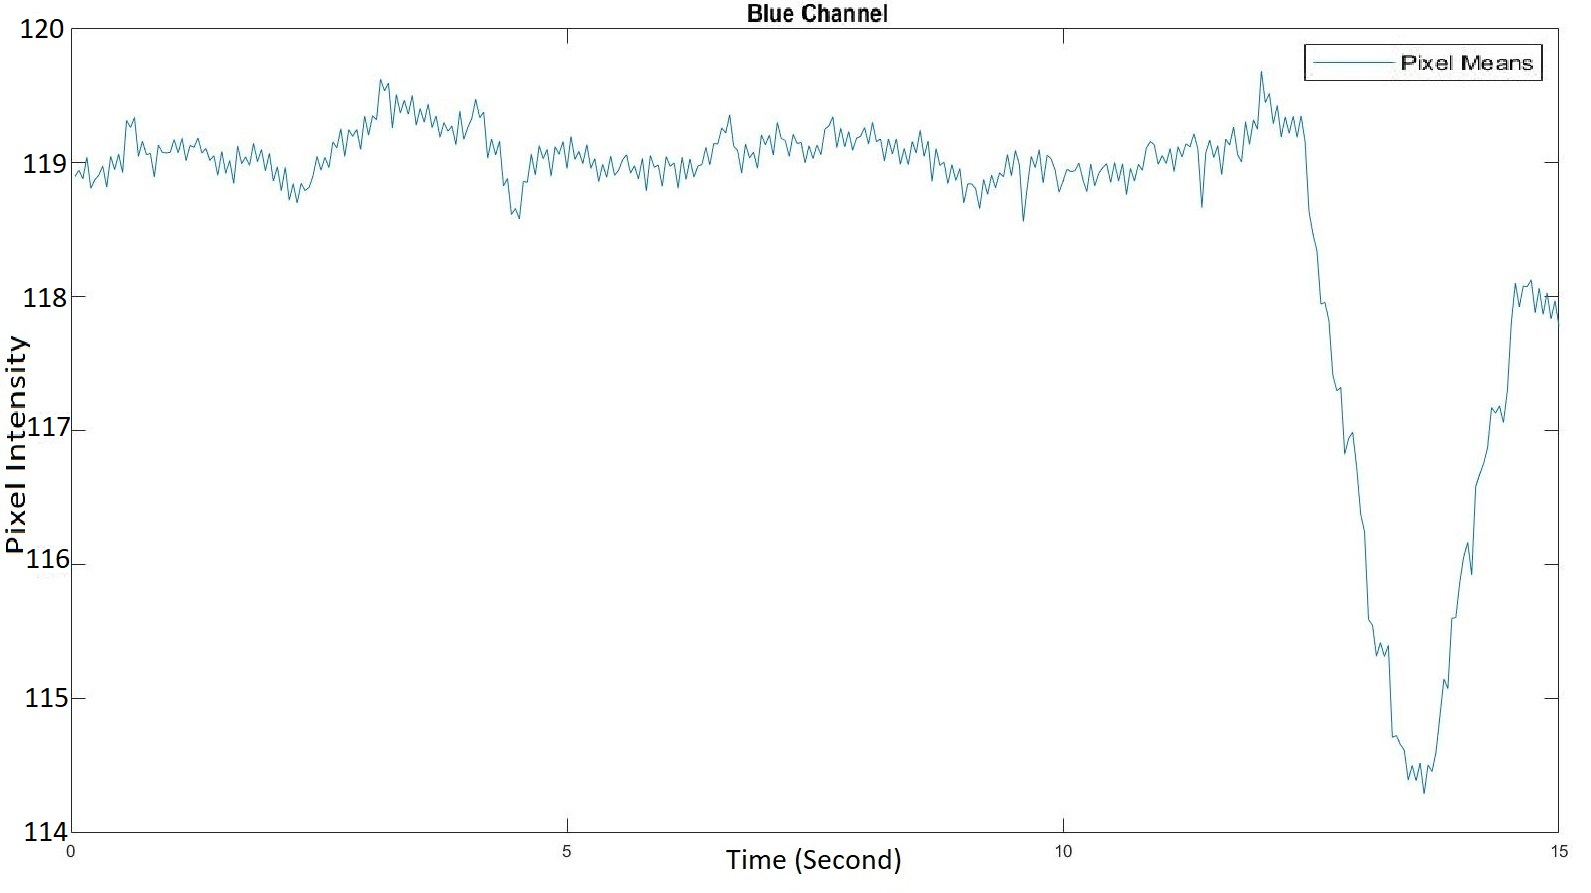
\includegraphics[width=\textwidth,height=0.25\textheight]{Blue_channel_wajah1-ori}
	\caption{Grafik kanal warna biru Wajah1 sebelum proses magnifikasi.}
	\label{fig:grafik-blue-wajah1}   
\end{figure}

Pada Gambar~\ref{fig:grafik-blue-wajah1} terlihat bahwa hasil ekstraksi sinyal pada kanal warna biru sebelum dilakukan proses magnifikasi belum dapat merepresentasikan sinyal PPG untuk menentukan nilai rata-rata detak jantung.

\begin{figure}[ht]
	\vspace{0.5em}
	\centering
	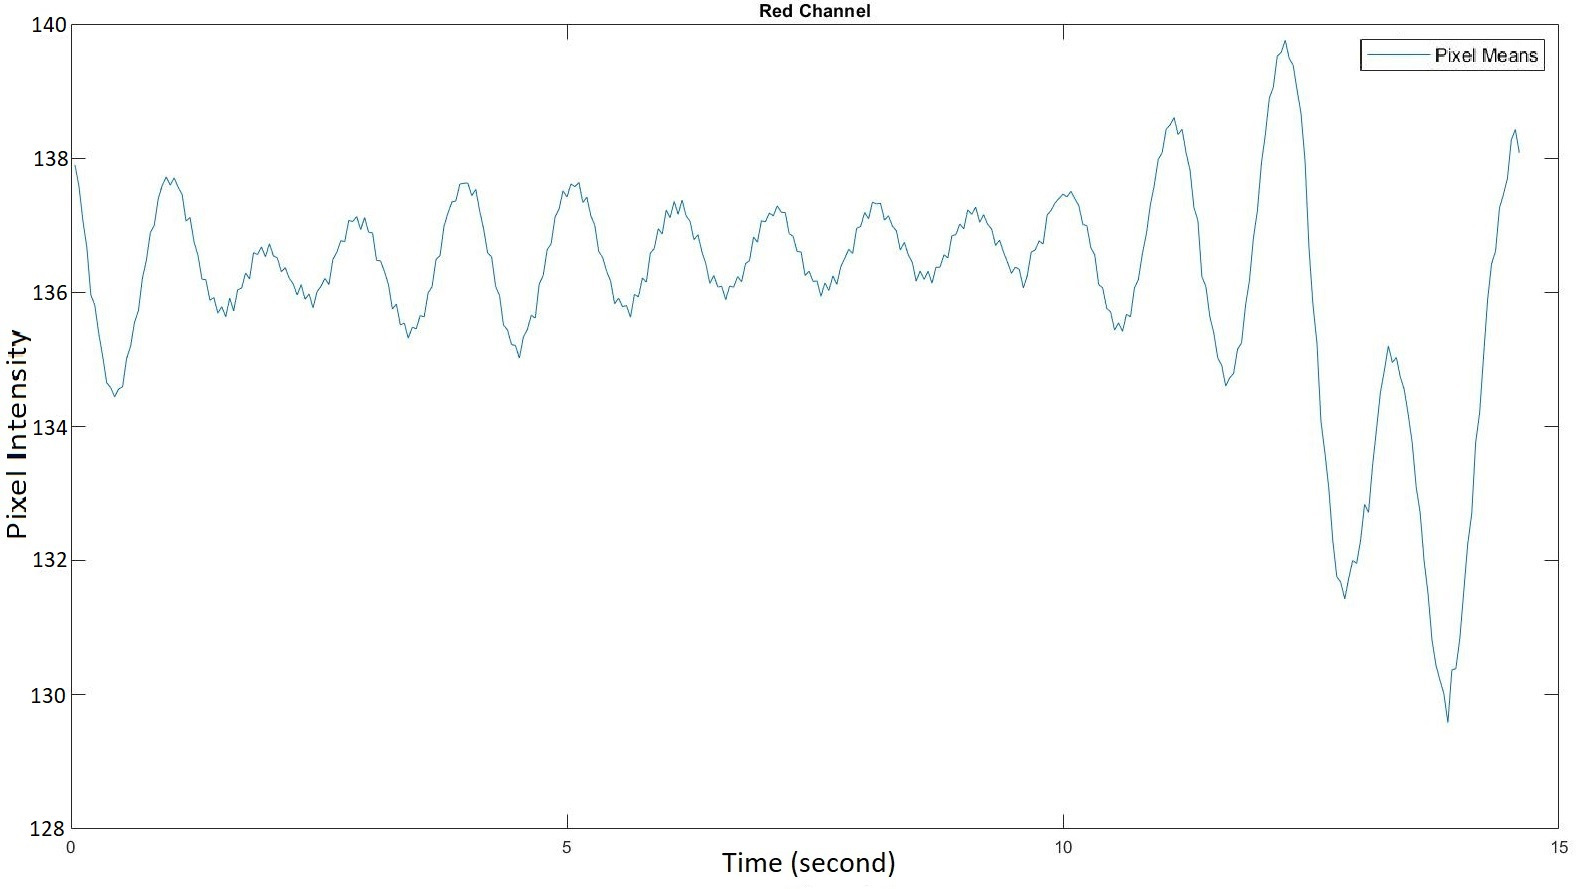
\includegraphics[width=\textwidth,height=0.25\textheight]{Red_channel_wajah1-result}
	\caption{Grafik kanal warna merah Wajah1 setelah proses magnifikasi.}
	\label{fig:grafik-red-wajah1-result}   
\end{figure}
Pada Gambar~\ref{fig:grafik-red-wajah1-result} terlihat bahwa hasil ekstraksi sinyal pada kanal warna merah setelah dilakukan proses magnifikasi mempunyai karakteristik gelombang sinusoidal yang dapat digunakan untuk merepresentasikan sinyal PPG untuk menentukan nilai rata-rata detak jantung.
\newpage
\begin{figure}[ht]
	\vspace{0.5em}
	\centering
	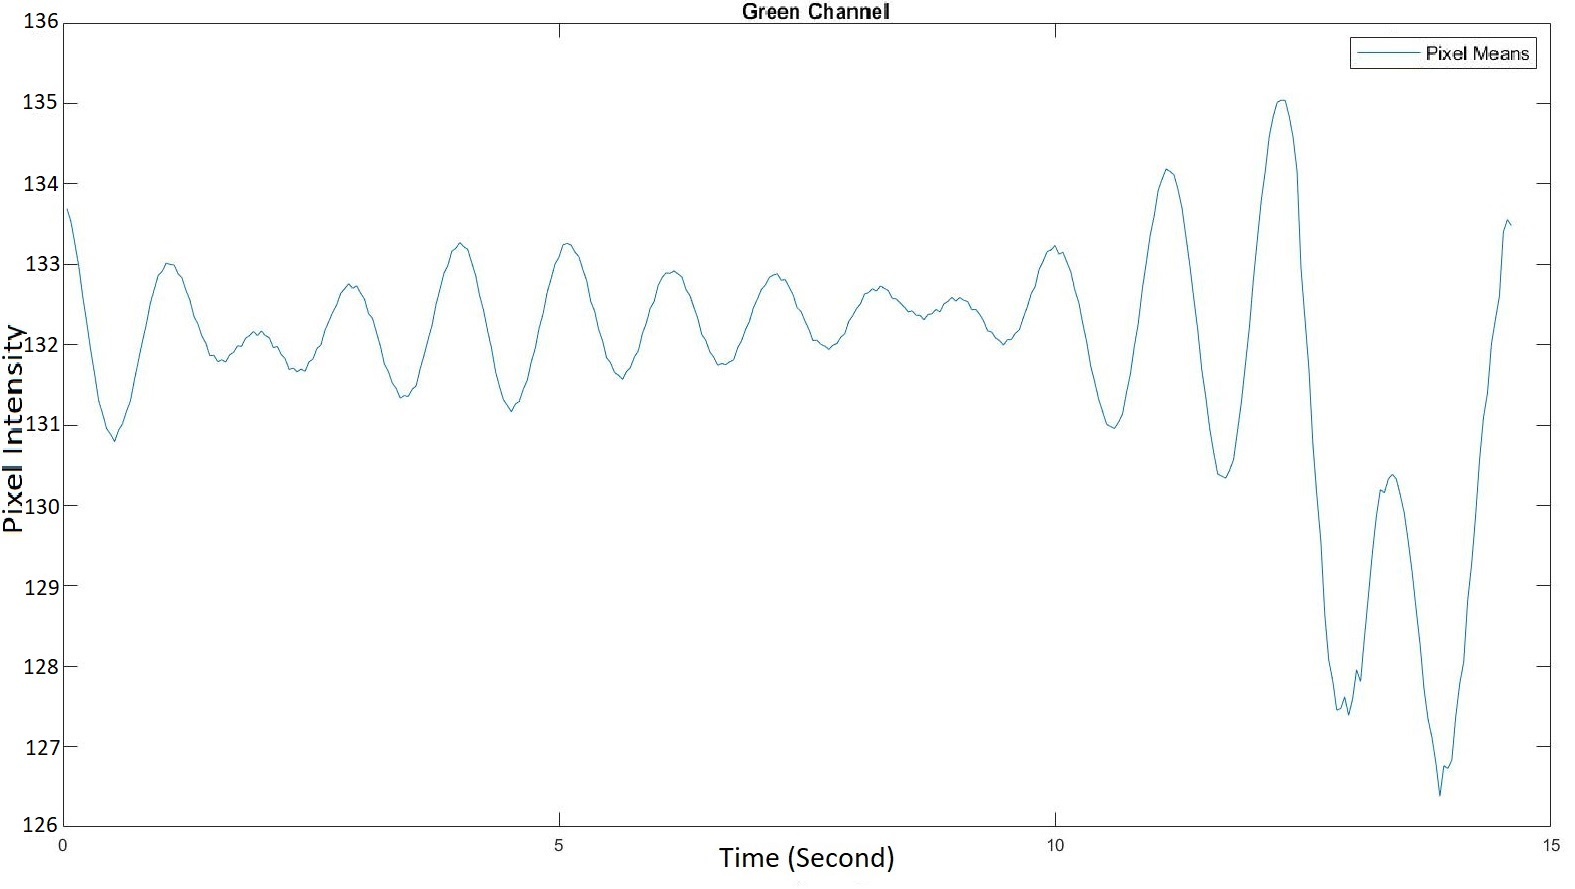
\includegraphics[width=\textwidth,height=0.25\textheight]{Green_channel_wajah1-result}
	\caption{Grafik kanal warna hijau Wajah1 setelah proses magnifikasi.}
	\label{fig:grafik-green-wajah1-result}   
\end{figure}
Pada Gambar~\ref{fig:grafik-green-wajah1-result} terlihat bahwa hasil ekstraksi sinyal pada kanal warna hijau setelah dilakukan proses magnifikasi mempunyai karakteristik gelombang sinusoidal yang dapat digunakan untuk merepresentasikan sinyal PPG untuk menentukan nilai rata-rata detak jantung.

\begin{figure}[ht]
	\vspace{0.5em}
	\centering
	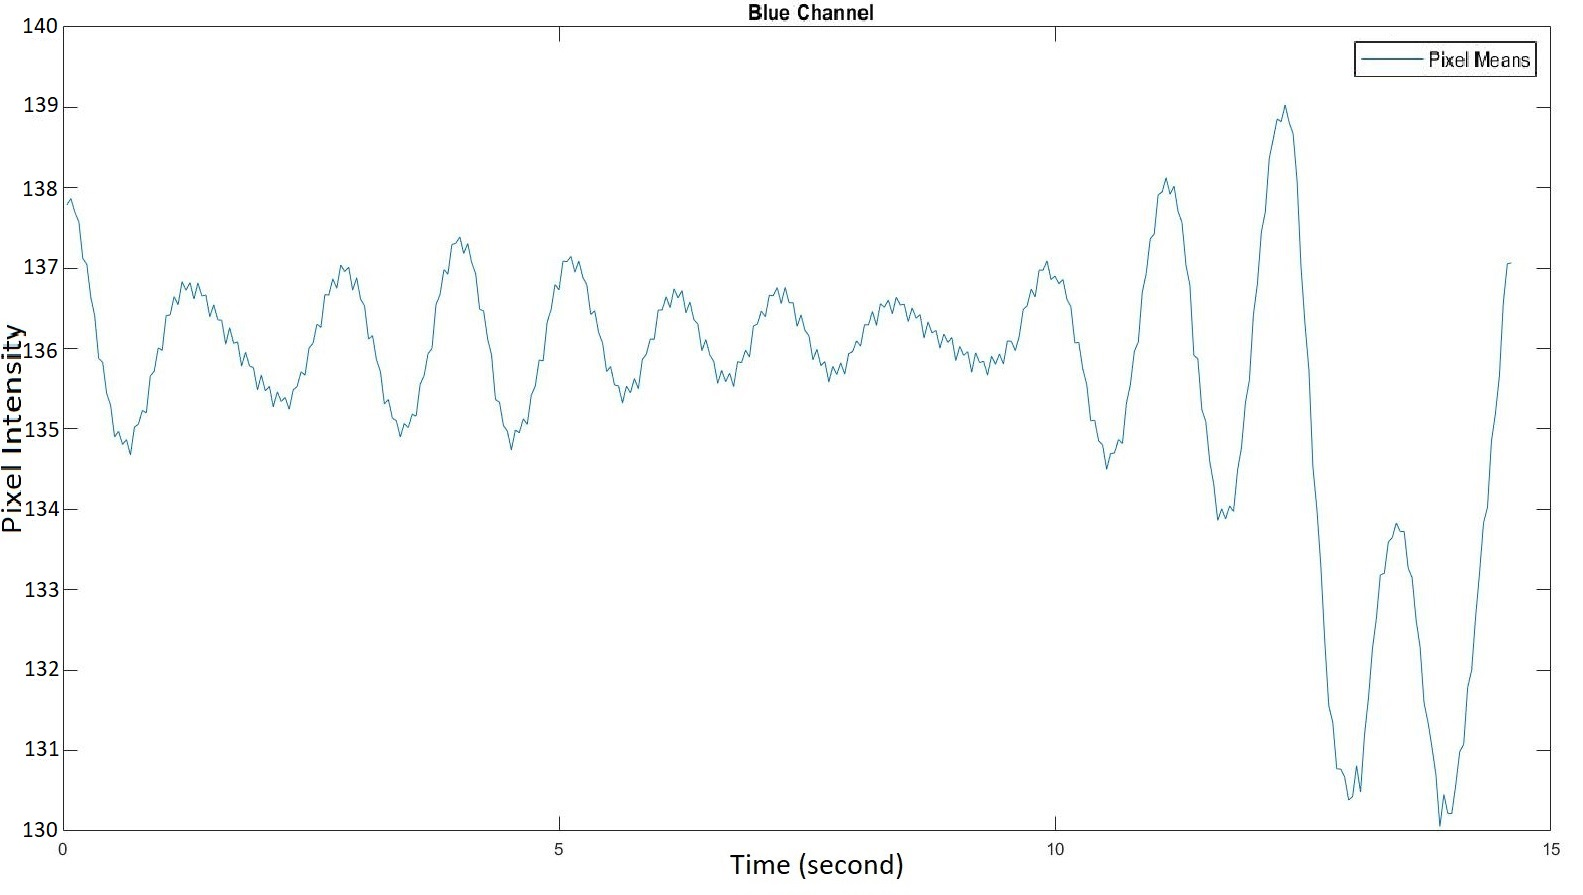
\includegraphics[width=\textwidth,height=0.25\textheight]{Blue_channel_wajah1-result}
	\caption{Grafik kanal warna biru Wajah1 setelah proses magnifikasi.}
	\label{fig:grafik-blue-wajah1-result}   
\end{figure}
Pada Gambar~\ref{fig:grafik-blue-wajah1-result} terlihat bahwa hasil ekstraksi sinyal pada kanal warna biru setelah dilakukan proses magnifikasi mempunyai karakteristik gelombang sinusoidal yang dapat digunakan untuk merepresentasikan sinyal PPG untuk menentukan nilai rata-rata detak jantung.
\newpage
\begin{figure}[ht]
	\vspace{0.5em}
	\centering
	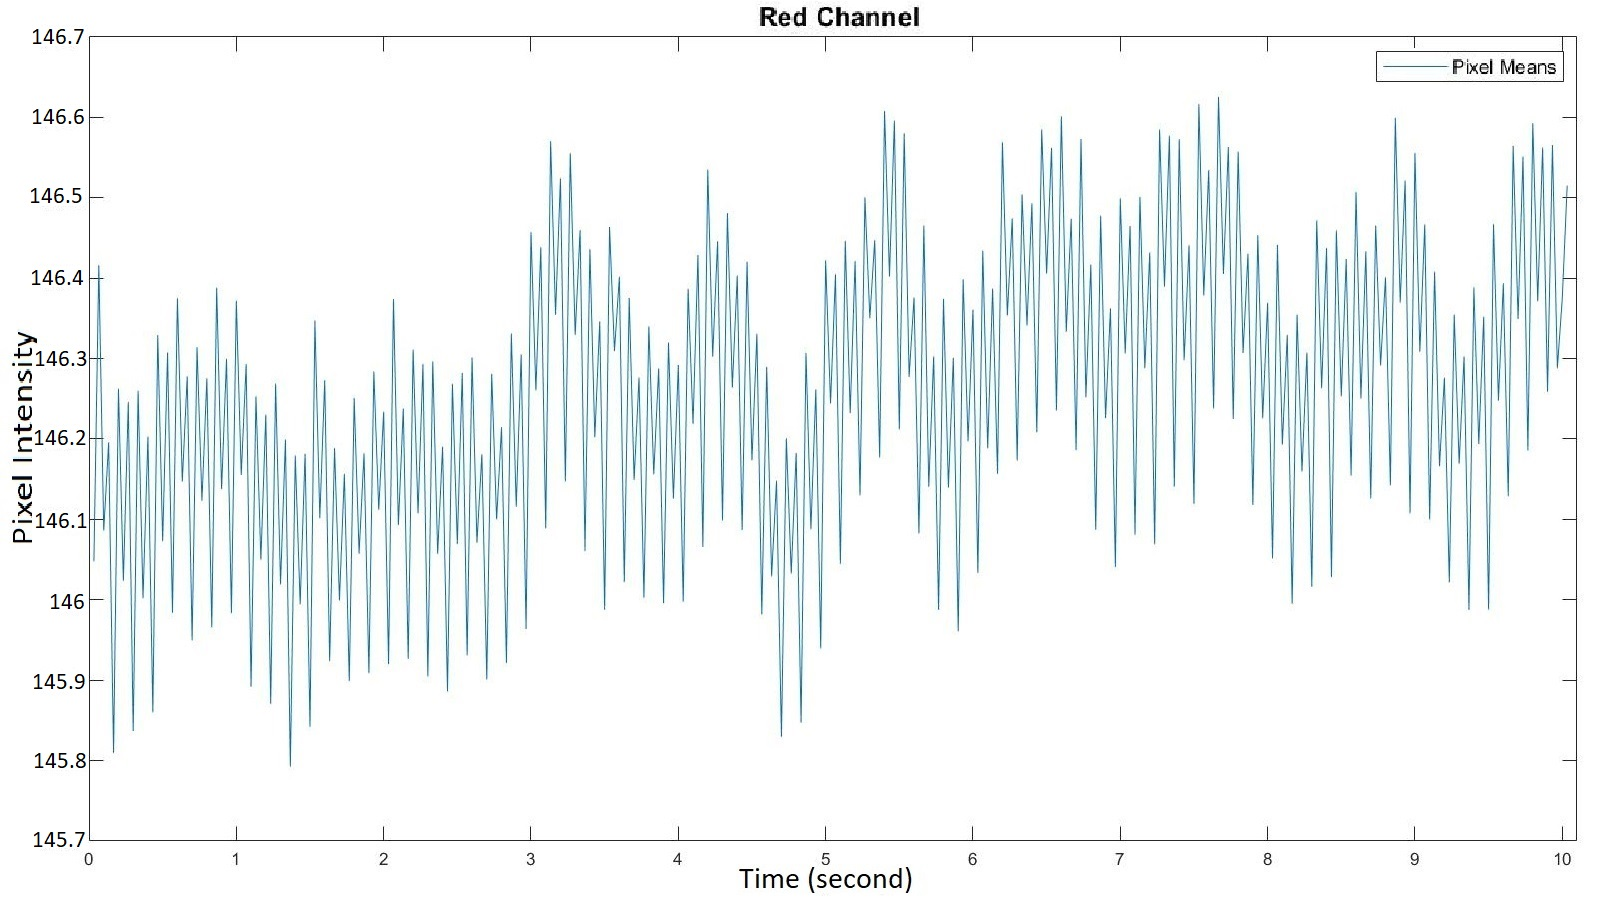
\includegraphics[width=\textwidth,height=0.25\textheight]{Red_channel_wajah2-ori}
	\caption{Grafik kanal warna merah Wajah2 sebelum proses magnifikasi.}
	\label{fig:grafik-red-wajah2}   
\end{figure}
Pada Gambar~\ref{fig:grafik-red-wajah2} terlihat bahwa hasil ekstraksi sinyal pada kanal warna merah sebelum dilakukan proses magnifikasi belum dapat merepresentasikan sinyal PPG untuk menentukan nilai rata-rata detak jantung.

\begin{figure}[ht]
	\vspace{0.5em}
	\centering
	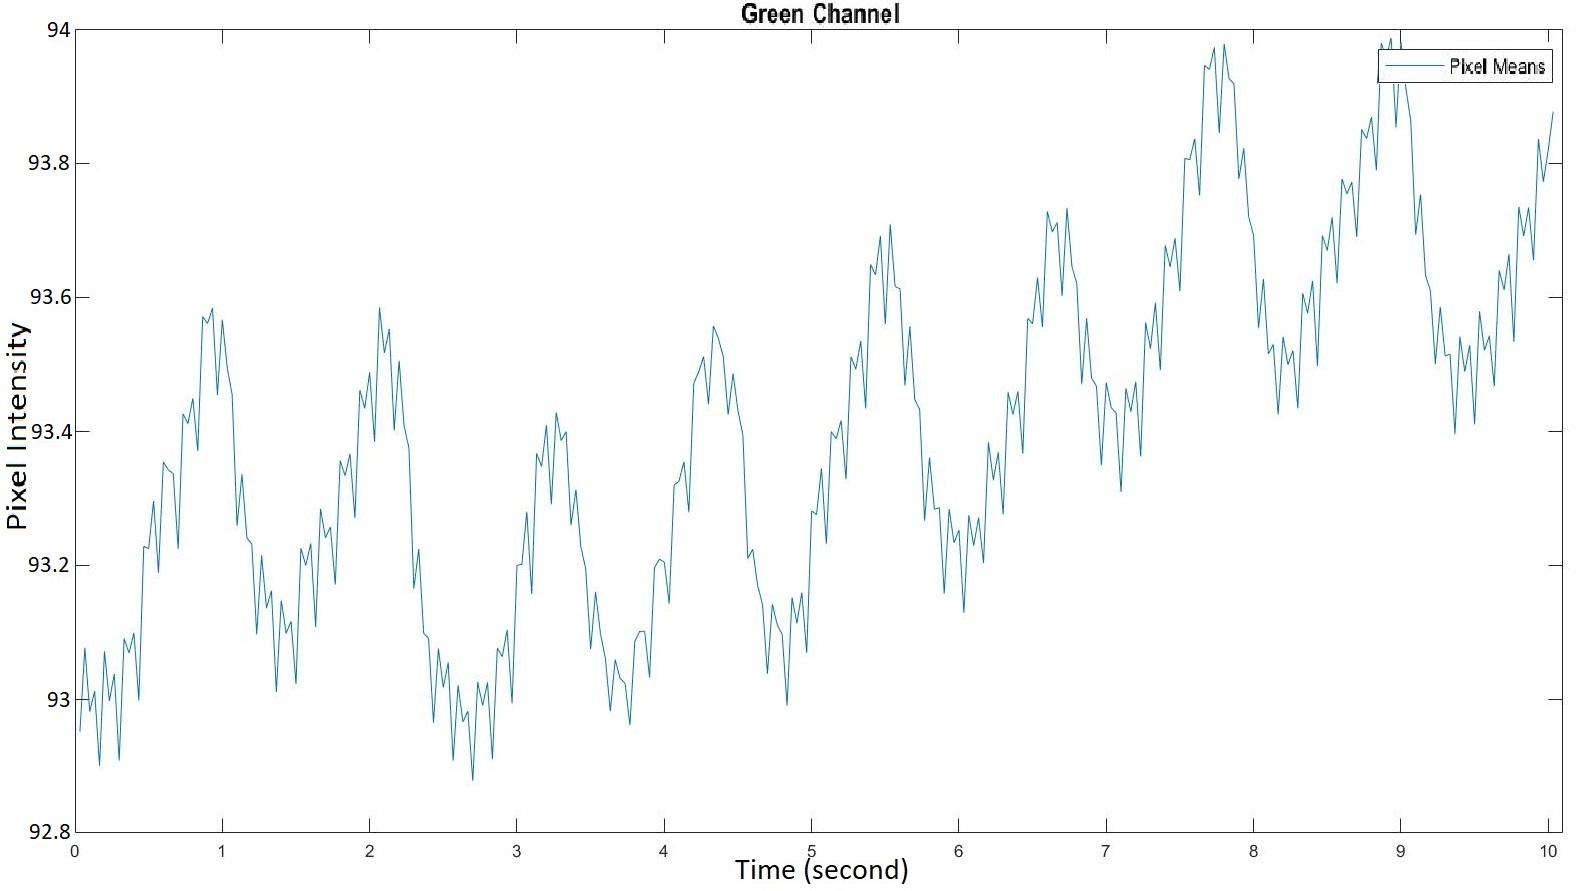
\includegraphics[width=\textwidth,height=0.25\textheight]{Green_channel_wajah2-ori}
	\caption{Grafik kanal warna hijau Wajah2 sebelum proses magnifikasi.}
	\label{fig:grafik-green-wajah2}   
\end{figure}
Pada Gambar~\ref{fig:grafik-green-wajah2} terlihat bahwa hasil ekstraksi sinyal pada kanal warna hijau sebelum dilakukan proses magnifikasi telah memiliki karakteristik bentuk gelombang periodik merepresentasikan sinyal PPG untuk menentukan nilai rata-rata detak jantung meskipun data yang dihasilkan tidak sebaik saat telah dilakukan proses magnifikasi.
\newpage
\begin{figure}[ht]
	\vspace{0.5em}
	\centering
	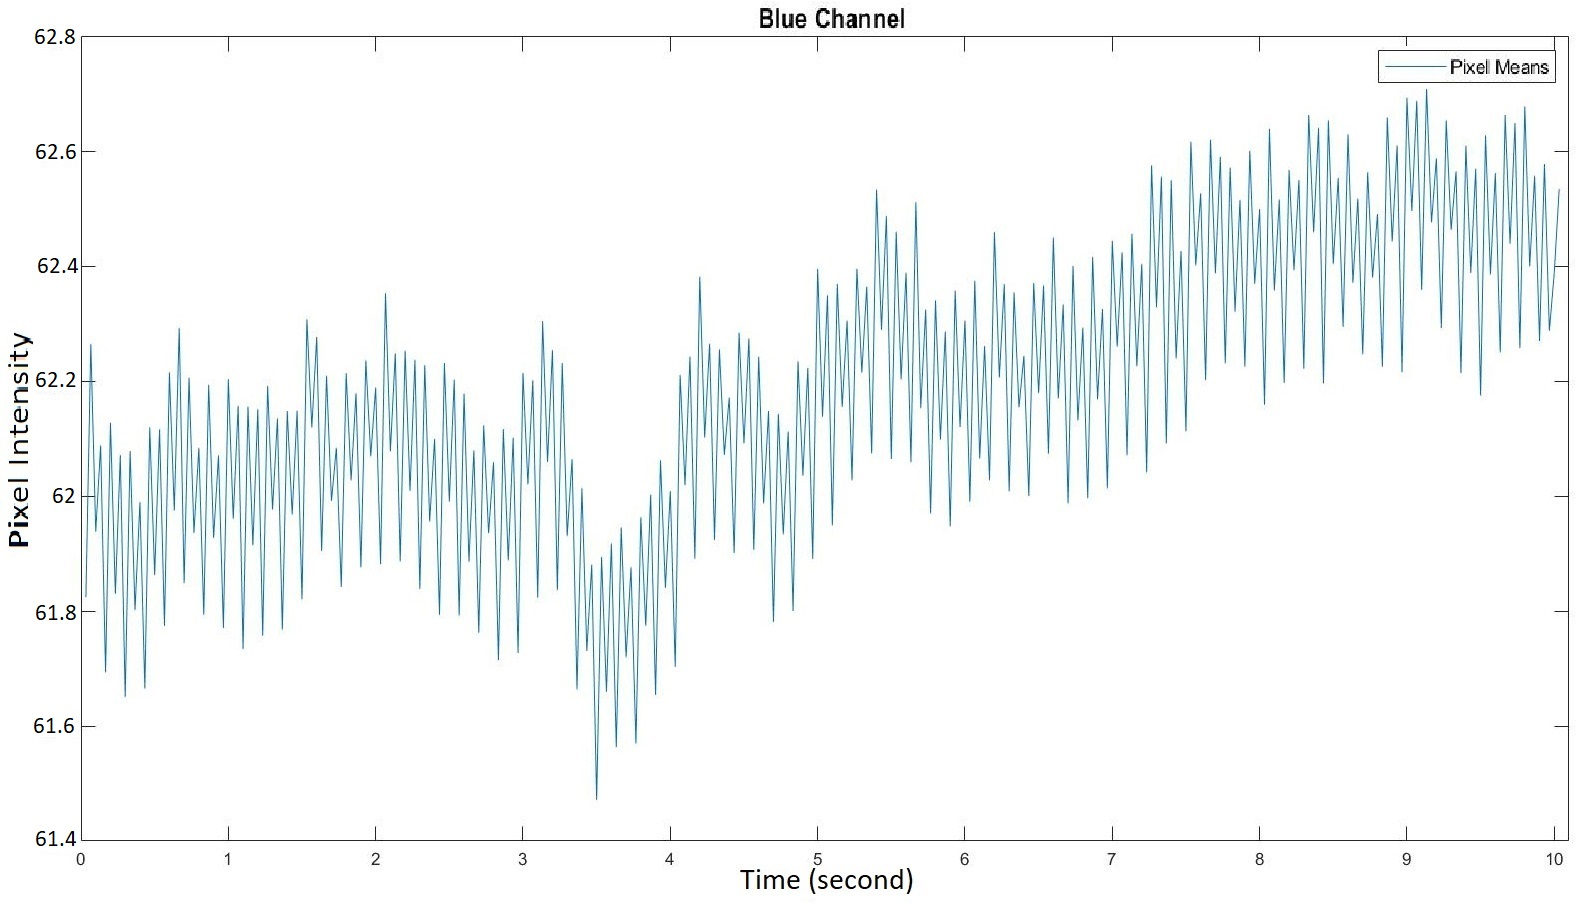
\includegraphics[width=\textwidth,height=0.25\textheight]{Blue_channel_wajah2-ori}
	\caption{Grafik kanal warna biru Wajah2 sebelum proses magnifikasi.}
	\label{fig:grafik-blue-wajah2}   
\end{figure}
Pada Gambar~\ref{fig:grafik-blue-wajah2} terlihat bahwa hasil ekstraksi sinyal pada kanal warna biru sebelum dilakukan proses magnifikasi belum dapat merepresentasikan sinyal PPG untuk menentukan nilai rata-rata detak jantung.

\begin{figure}[ht]
	\vspace{0.5em}
	\centering
	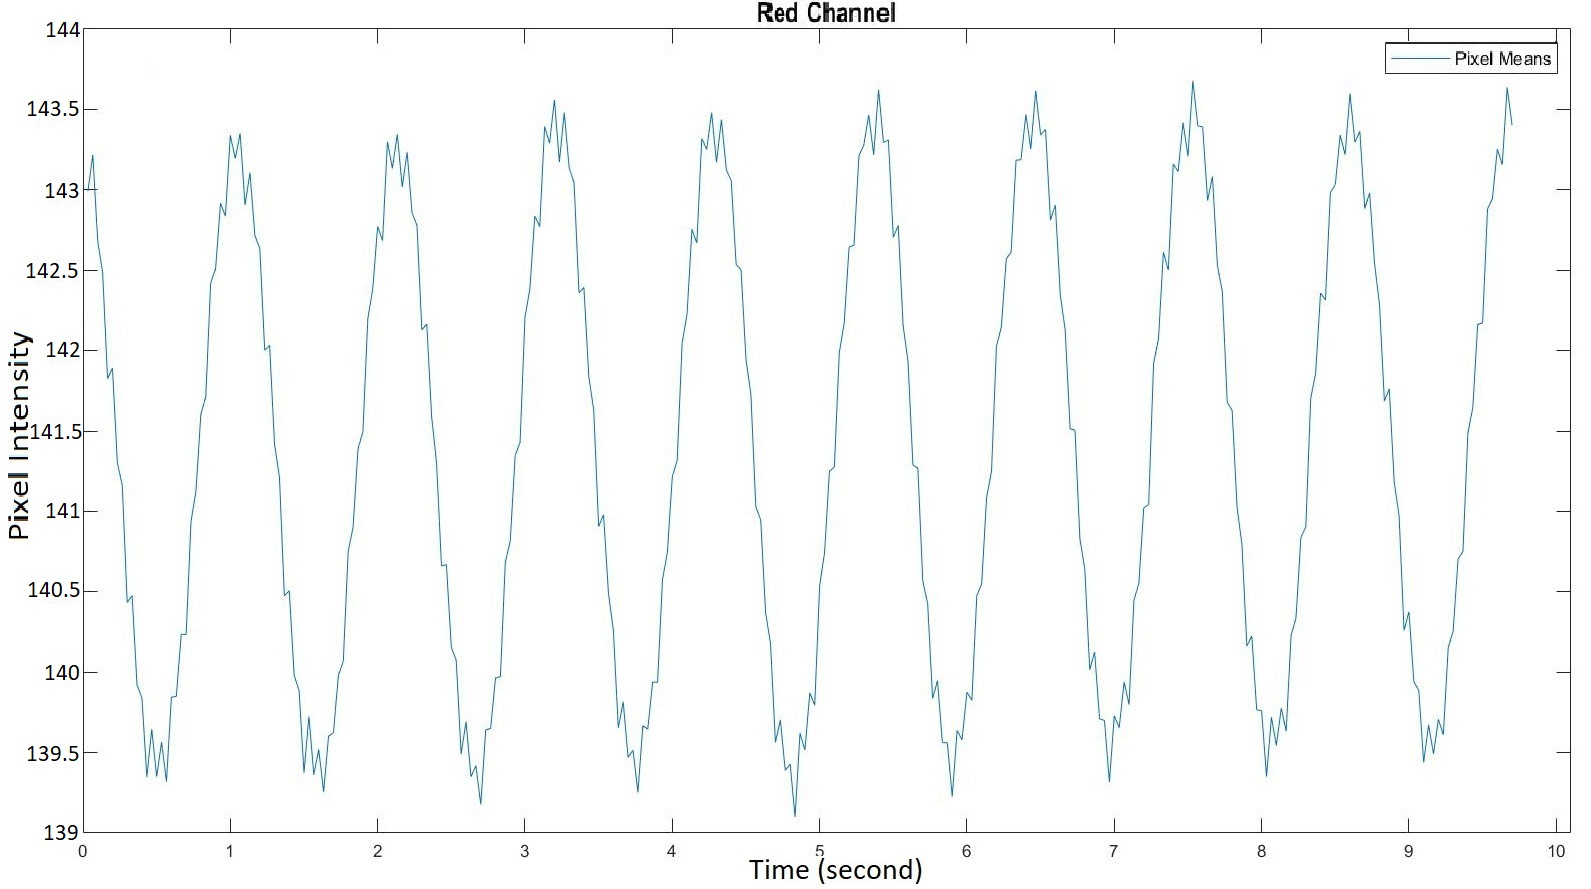
\includegraphics[width=\textwidth,height=0.25\textheight]{Red_channel_wajah2-result}
	\caption{Grafik kanal warna merah Wajah2 setelah proses magnifikasi.}
	\label{fig:grafik-red-wajah2-result}   
\end{figure}
Pada Gambar~\ref{fig:grafik-red-wajah2-result} terlihat bahwa hasil ekstraksi sinyal pada kanal warna merah setelah dilakukan proses magnifikasi mempunyai karakteristik gelombang sinusoidal yang dapat digunakan untuk merepresentasikan sinyal PPG untuk menentukan nilai rata-rata detak jantung.
\newpage
\begin{figure}[ht]
	\vspace{0.5em}
	\centering
	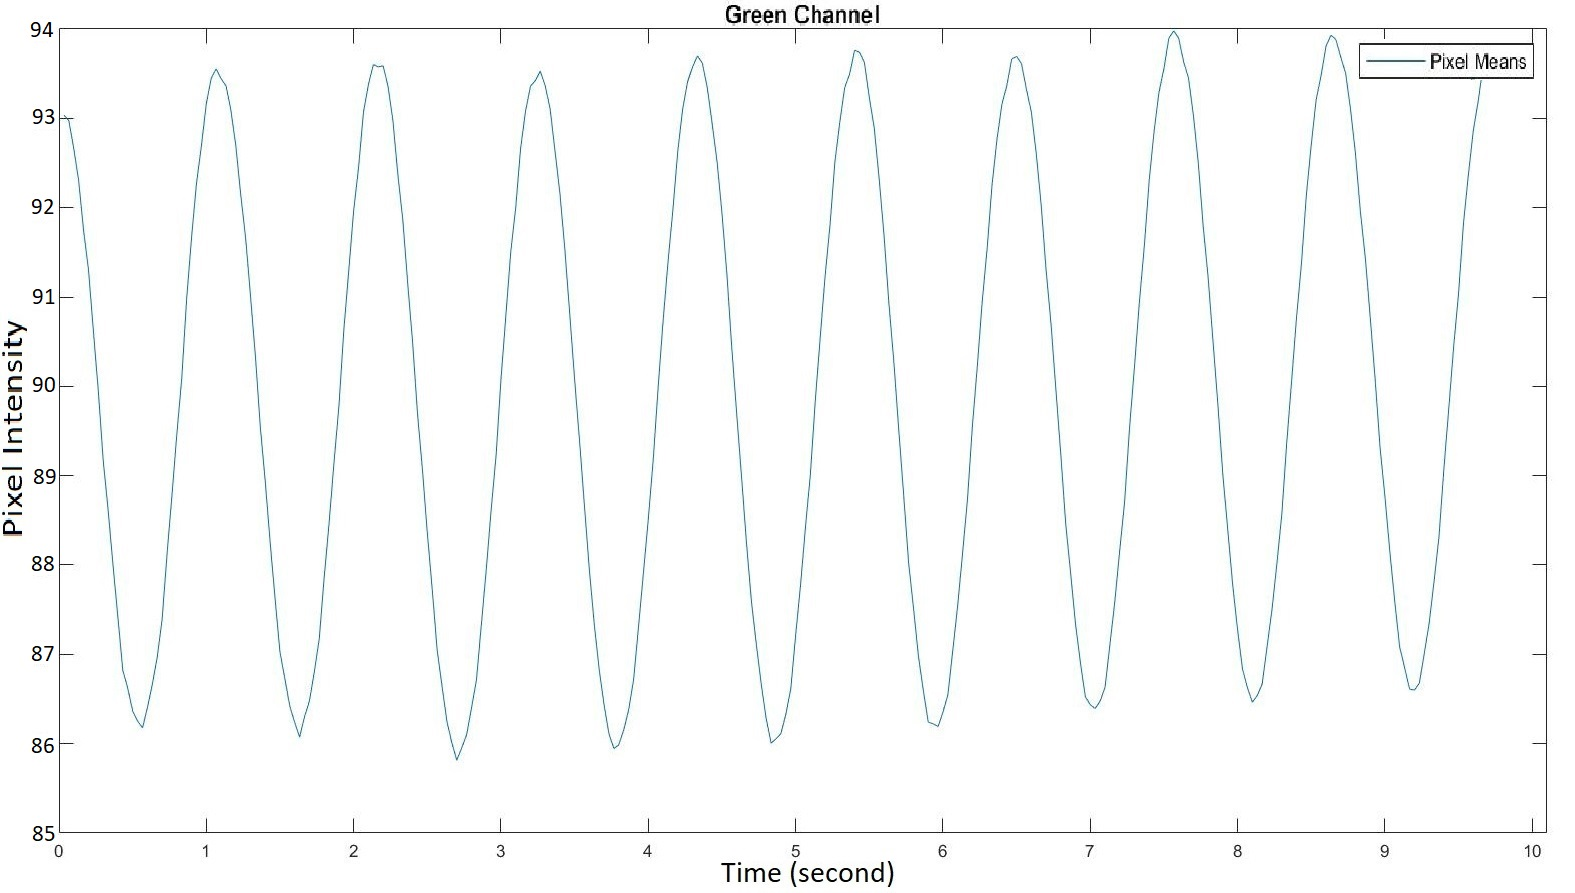
\includegraphics[width=\textwidth,height=0.25\textheight]{Green_channel_wajah2-result}
	\caption{Grafik kanal warna hijau Wajah2 setelah proses magnifikasi.}
	\label{fig:grafik-green-wajah2-result}   
\end{figure}
Pada Gambar~\ref{fig:grafik-green-wajah2-result} terlihat bahwa hasil ekstraksi sinyal pada kanal warna hijau setelah dilakukan proses magnifikasi mempunyai karakteristik gelombang sinusoidal yang dapat digunakan untuk merepresentasikan sinyal PPG untuk menentukan nilai rata-rata detak jantung.

\begin{figure}[ht]
	\vspace{0.5em}
	\centering
	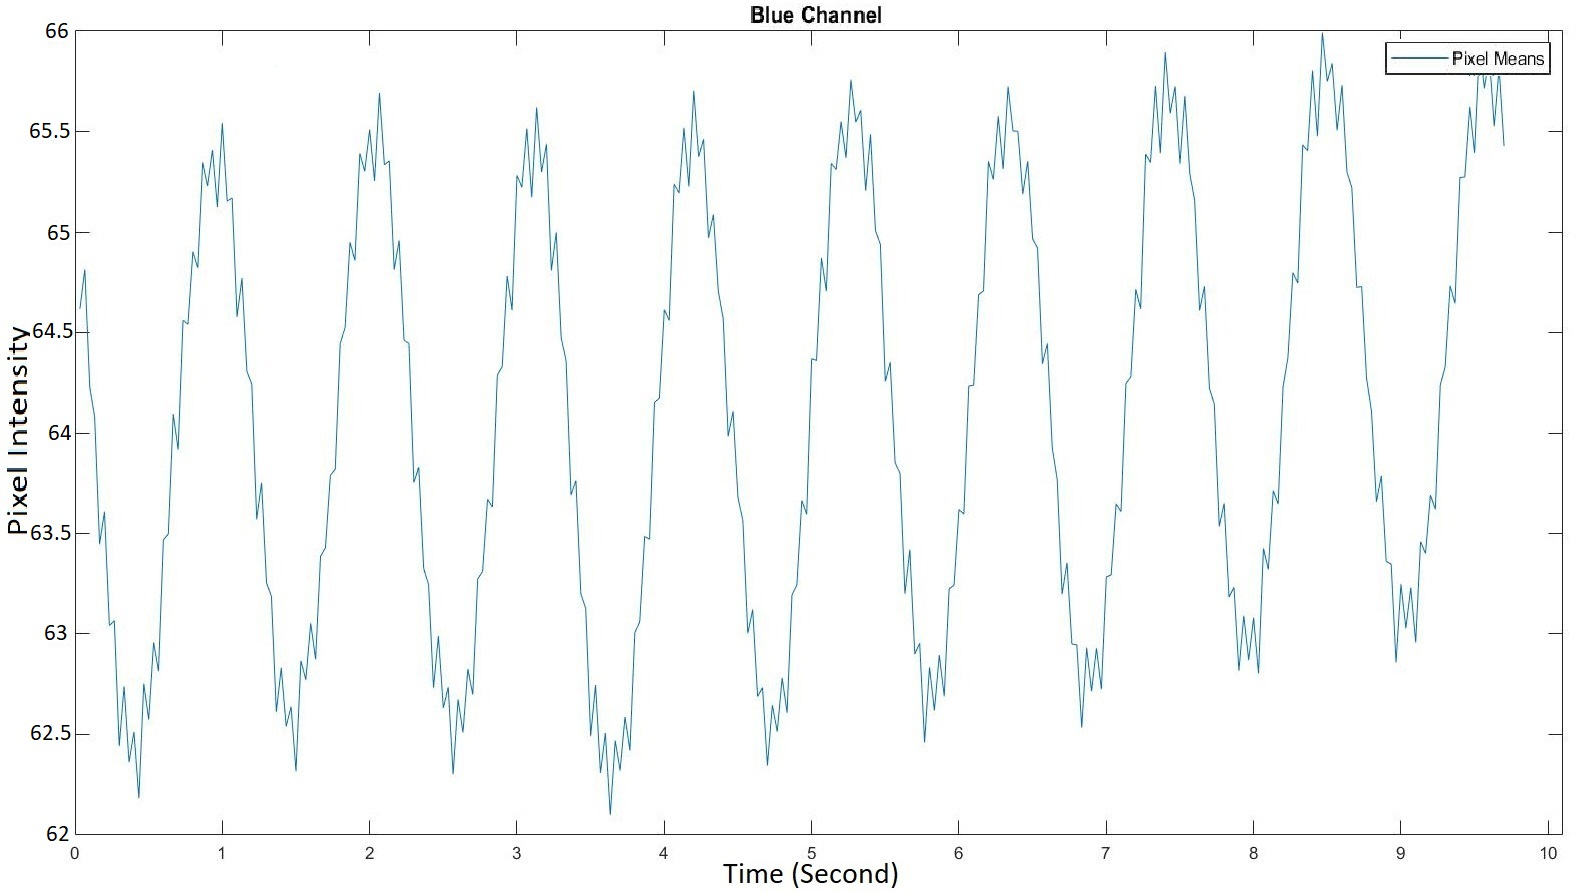
\includegraphics[width=\textwidth,height=0.25\textheight]{Blue_channel_wajah2-result}
	\caption{Grafik kanal warna biru Wajah2 setelah proses magnifikasi.}
	\label{fig:grafik-blue-wajah2-result}   
\end{figure}
Pada Gambar~\ref{fig:grafik-blue-wajah2-result} terlihat bahwa hasil ekstraksi sinyal pada kanal warna biru setelah dilakukan proses magnifikasi mempunyai karakteristik gelombang sinusoidal yang dapat digunakan untuk merepresentasikan sinyal PPG untuk menentukan nilai rata-rata detak jantung.
\newpage
\section{Pengujian nilai detak jantung dari hasil ekstraksi sinyal}
Pada proses pengujian ini dilakukan pengambilan data pada daerah sekitar wajah dari 10 orang berbeda untuk kemudian diproses menjadi data detak jantung.~Hasil pengujian yang didapatkan akan dibandingkan dengan alat lain yang dapat digunakan untuk mengukur detak jantung yaitu pulse oximeter dan xiaomi mi band 3 yang merupakan produk-produk komersil yang telah beredar luas.~Proses validasi dilakukan dengan cara mengambil data pada subyek secara bersamaan dengan kamera dan alat-alat yang digunakan untuk validasi, sehingga data yang diperoleh dapat dibandingkan dengan baik.

\begin{figure}[ht]
	\vspace{0.5em}
	\centering
	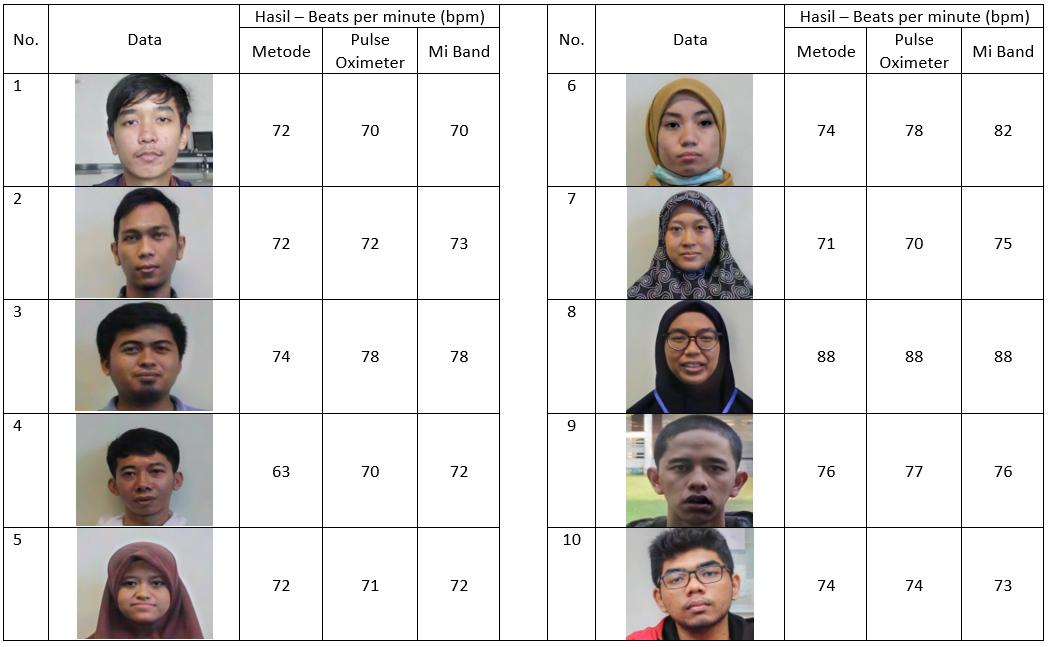
\includegraphics[width=\textwidth]{data10}
	\caption{Data hasil detak jantung (HR) yang diperoleh}
	\label{fig:data1}   
\end{figure}

Gambar~\ref{fig:data1} merupakan hasil percobaan ekstraksi nilai detak jantung yang didapatkan dari 10 sampel data yang berbeda.~Pada kolom metode merupakan hasil ekstraksi yang didapatkan dengan algoritma yang digunakan untuk mengerjakan proyek akhir, sedangkan kolom pulse oximeter dan mi band merupakan hasil yang didapatkan dari alat validasi.~Pengukuran nilai HR dari metode yang digunakan dilakukan dalam waktu sampling sekitar 15 detik, untuk pengukuran dengan mi band juga diperlukan waktu 15 detik namun data yang ditampilkan tidak berisifat kontinu dalam artian pengukuran tidak dilakukan secara terus-menerus, sedangkan untuk pengukuran menggunakan pulse oximeter waktu minimal yang diperlukan adalah 5 detik dan pengukuran dapat dilakukan secara kontinu.

\subsection{Hasil dan Analisa}
Berdasarkan data hasil ektraksi nilai HR pada Gambar~\ref{fig:data1} dapat ditemukan hasil yang identik dari ketiga pengujian dengan nilai 88 bpm pada data ke-8, sedangkan data ke-3 merupakan data dengan nilai error paling besar dengan selisih hingga 9 bpm.~Hasil pengujian lainnya mempunyai nilai error yang bervariasi sebesar \(\pm\) 0-4 bpm.
%\section{ Pengujian Pemfilteran Sinyal}
%\section{ Hasil Pengujian Menggunakan Sistem Embedded}